\begin{figure}[!hbt]
  \centering
  \subfigure{
    \label{fig:optimize-subrefine--8020}
    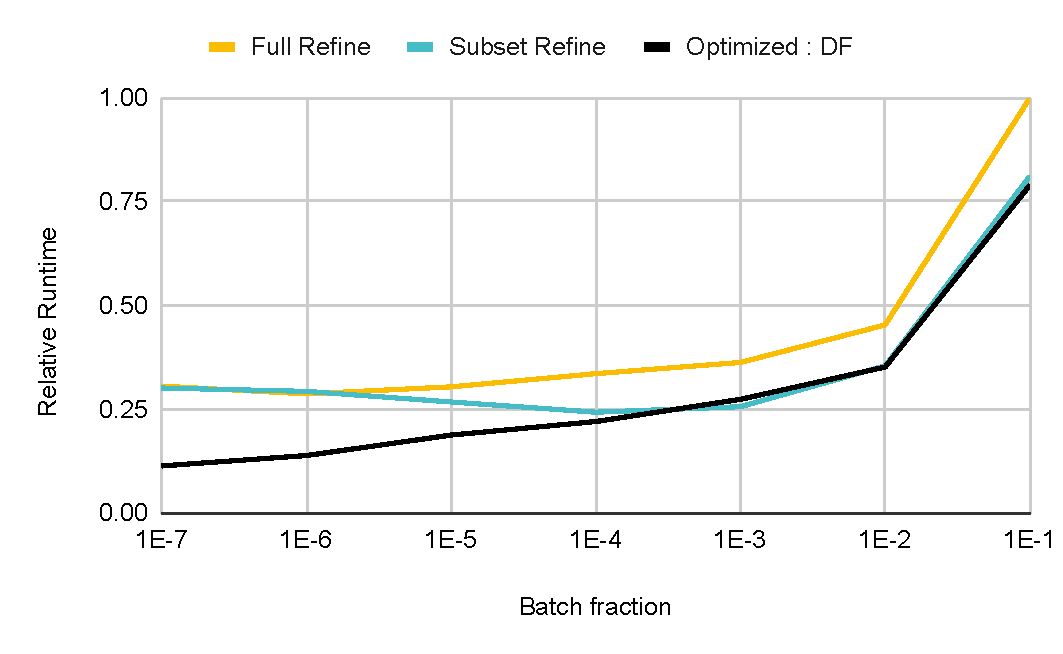
\includegraphics[width=0.98\linewidth]{out/optimize-subrefine-8020.pdf}
  } \\[-2ex]
  \caption{Mean Runtime and Modularity of communities obtained with our multicore implementation of \textit{Static}, \textit{Naive-dynamic (ND)}, \textit{Delta-screening (DS)}, and \textit{Dynamic Frontier (DF)} Leiden on real-world dynamic graphs, using batch updates of size $10^{-5}|E_T|$ to $10^{-3}|E_T|$. Here, (a) and (b) display the overall runtime and modularity across all temporal graphs, while (c) and (d) display the runtime and modularity for each individual graph. In (a), the speedup of each approach relative to Static Leiden is labeled.}
  \label{fig:optimize-subrefine}
\end{figure}
